\documentclass[a4paper]{article}

\usepackage[utf8]{inputenc}
\usepackage[T1]{fontenc}
\usepackage{textcomp}
\usepackage[english]{babel}
\usepackage{amsmath, amssymb}


%figure support
\usepackage{import}
\usepackage{xifthen}
\pdfminorversion=7
\usepackage{pdfpages}
\usepackage{transparent}
\newcommand{\incfig}[1]{%
	\def\svgwidth{\columnwidth}
	\import{./figures/}{#1.pdf_tex}
}
\graphicspath{ {./figures/} }
\pdfsuppresswarningpagegroup=1

\begin{document}
	\title{CEN4088.01 Lab 5 Due 10/24/19}
	\author{Brandon Thompson 5517}
	\maketitle

	\begin{figure}[ht!]
		\centering
		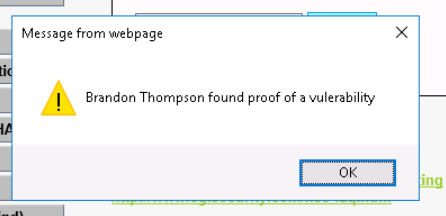
\includegraphics[width=0.8\textwidth]{1_2_5}
		\caption{Part 1: Exposed XSS vulnerability. DVWA security set to low.}
		\label{fig:1_2_5}
	\end{figure}
	When the DVWA security is set to high the text box takes whatever input it is
	given and converts it to a string so that special characters do not conflict
	with the code of the text output.\\
	
	SQL injection attack, input \texttt{a' ORDER BY 1;\#} in the User ID field.
	Outputs a single first name and surname pair. When \texttt{a' ORDER BY 2;\#}
	is passed to the input, outputs a single first name and surname pair.
	When \texttt{a' ORDER BY 3;\#} is passed result is an error message:
	''Unknown column '3' in 'order caluse'.'' This shows that there are 2 columns
	in the database.
	\begin{figure}[ht!]
		\centering
		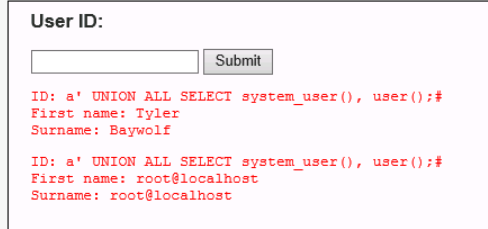
\includegraphics[width=0.8\textwidth]{1_3_19}
		\caption{Part 1: User account information.}
		\label{fig:1_3_19}
	\end{figure}

	\begin{figure}[ht!]
		\centering
		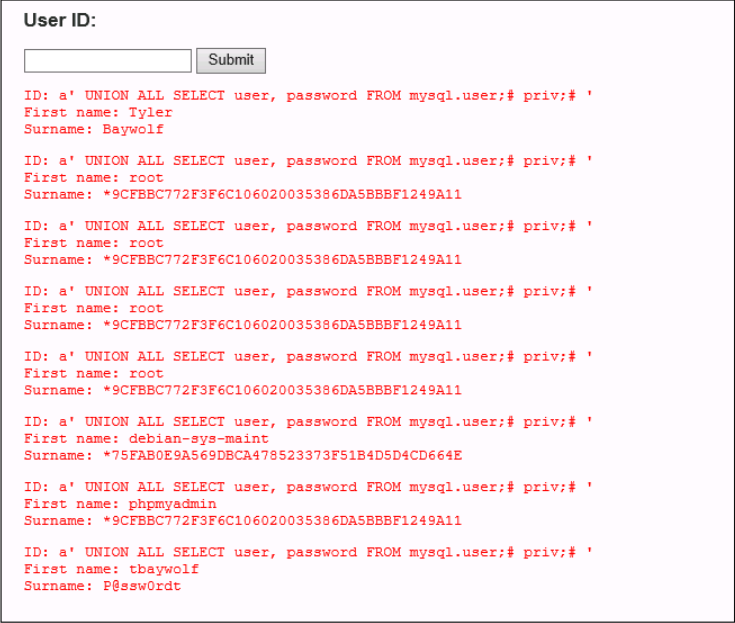
\includegraphics[width=0.8\textwidth]{1_3_21}
		\caption{Part 1: Database hash information}
		\label{fig:1_3_21}
	\end{figure}
	% Describe the purpose of hashing in a database
	
	Hashing generates a key related to the item being hashed. This key is shorter
	than the original value and thus makes it easier to find items based on their
	hashed key.\\

	\begin{figure}[ht!]
		\centering
		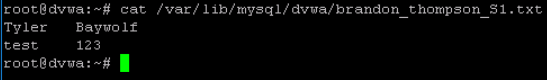
\includegraphics[width=0.8\textwidth]{1_4_3}
		\caption{Contents of \texttt{brandon\_thompson\_S1.txt}}
		\label{fig:1_4_3}
	\end{figure}

	%Describe security countermeasures to mitigate the risk from compromise and
	%exploitation.
	Sanitizing the inputs so that no special characters can be used will remove the
	vulnerability of the system by not allowing the user to input malicious code.
	If the system is compromised, not allowing file write/execute permissions will
	not allow users to create documents or execute scripts.
	\clearpage
	\begin{figure}[ht!]
		\centering
		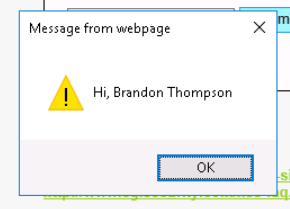
\includegraphics[width=0.8\textwidth]{2_2_5}
		\caption{Part 2: Exposed XSS vulnerability. DVWA security set to low.}
		\label{fig:2_2_5}
	\end{figure}

	Question 2.2.9 answered in part 1.\\
	
	Question 2.3.7 answered in part 1.\\
	\begin{figure}[ht!]
		\centering
		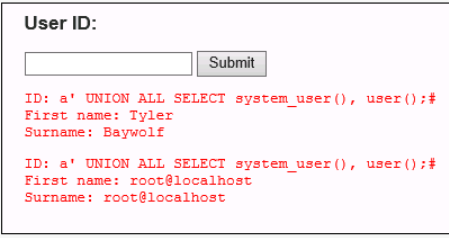
\includegraphics[width=0.8\textwidth]{2_3_16}
		\caption{Part 2: User information from SQL injection.}
		\label{fig:2_3_17}
	\end{figure}
	\clearpage
	\begin{figure}[ht!]
		\centering
		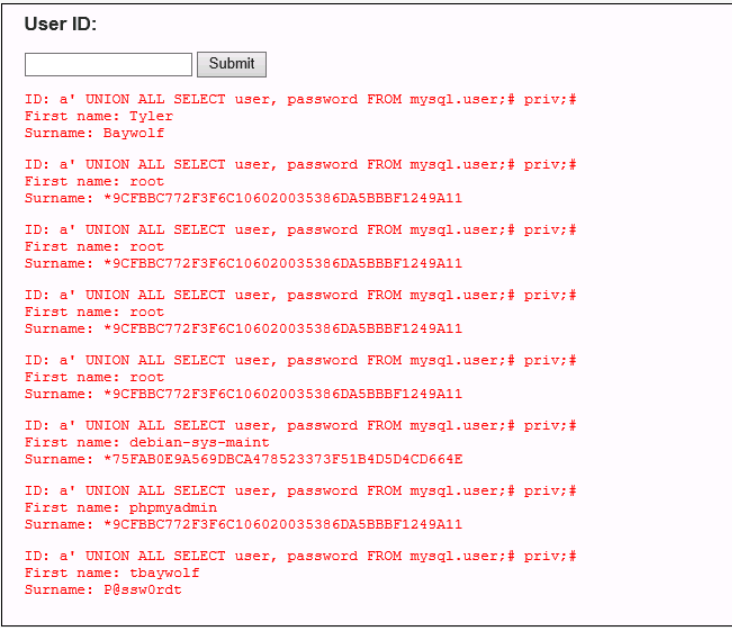
\includegraphics[width=0.8\textwidth]{2_3_18}
		\caption{Part 2: Database hash information from SQL injection.}
		\label{fig:2_3_18}
	\end{figure}

	Question 2.3.19 answered in part 1.\\

	\begin{figure}[ht!]
		\centering
		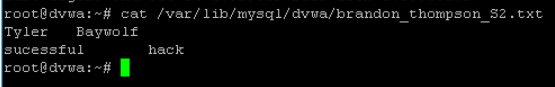
\includegraphics[width=0.8\textwidth]{2_4_3}
		\caption{Contents of \texttt{brandon\_thompson\_S2.txt}}
		\label{fig:2_4_3}
	\end{figure}
	
	Question 2.4.5 answered in part 1.
\end{document}
